\graphicspath{{chapter_3}}
\chapter[Laparoscopic Camera Motion Extraction]{Laparoscopic Camera Motion Extraction from Dynamic Surgical Scenes}
\chaptermark{Camera Motion Extraction}
\label{chap:camera_motion_extraction}
\minitoc

\paragraph{Disclaimer} This \chapref{chap:camera_motion_extraction} is an \textit{in extenso} reproduction of \cite{huber2022deep}. Only \secref{c3:sec:introduction} was adapted to highlight additional context within the scope of this thesis.

\newpage

\section{Introduction}
\label{c3:sec:introduction}
% short introduction to deep learning in medical imaging
% The advancement of dedicated chips unlocked the application of Deep Neural Networks (DNN) to vast datasets, and with it, the extraction of previously intangible information from them. As a result, DNNs lead to dramatic SOTA improvements in 
The goal in IL is to learn an expert policy from a set of expert demonstrations.
% $\pi_\text{E}: s_t \rightarrow a_t$ that maps a state $s_t$ to an action $a_t$ at timestep $t$, with action-state pairs drawn from a trajectory $\tau_i = \{(s_t,a_t),...,(s_{t+T-1},a_{t+T-1})\}$, sampled from expert demonstrations $\tau_i \in D$.
IL has been slow to transition to interventional imaging. In particular, the slow transition of modern IL methods into automating laparoscopic camera motion is due to a lack state-action-pair data \cite{kassahun2016surgical, esteva2019guide}. The need for automated laparoscopic camera motion \cite{pandya2014review, ellis2016task} has, therefore, historically sparked research in rule-based approaches that aim to reactively center surgical tools in the field of view \cite{agustinos2014visual, da2020scan}. DNNs could contribute to this work by facilitating SOTA tool segmentations and automated tool tracking \cite{garcia2017toolnet, garcia2021image, gruijthuijsen2021autonomous}.

% Widely available, and well curated datasets then quickly enabled the adaptation of DNNs to the medical imaging domain, facilitating assisted or fully automated image analysis, e.g. for diagnosis or segmentation. This progress, however, is slow to transition to the realm of interventional imaging, where automation faces dynamic environments and contextual dependencies \cite{vercauteren2019cai4cai}, in general. 

% In particular, the slow transition of DNNs into automating laparoscopic camera motion in Minimally Invasive Surgery (MIS) can be accounted for by a lack of task-specific data \cite{kassahun2016surgical, esteva2019guide}. The need for automated laparoscopic camera motion \cite{pandya2014review, ellis2016task} has, therefore, historically sparked research in rule-based approaches that, in their simplest form, aim at reactively centering surgical tools in the field of view (TODO: add citations). DNNs contribute to this work by facilitating SOTA tool segmentations for the identification of tool tips. 

Recent research contextualizes laparoscopic camera motion with respect to (w.r.t.) the user and the state of the surgery. DNNs could facilitate contextualization, as indicated by research in surgical phase and skill recognition \cite{kitaguchi2020real}. However, current contextualization is achieved through handcrafted rule-based approaches \cite{rivas2014towards, rivas2017smart}, or through stochastic modeling of camera positioning w.r.t. the tools \cite{weede2011intelligent, rivas2019transferring}. While the former do not scale well and are prone to nonlinear interventions, the latter only consider surgical tools. However, clinical evidence suggests camera motion is also caused by the surgeon's desire to observe tissue \cite{ellis2016task}. Non-rule-based, i.e. IL, attempts that consider both, tissue, and tools as source for camera motion are \cite{ji2018learning, su2020multicamera, wagner2021learning}, but they utilize an oversimplified setup, require multiple cameras or tedious annotations.

In current laparoscopic camera motion automation, DNNs merely solve auxiliary tasks. Consequentially, current laparoscopic camera motion automation is rule-based, and disregards tissue. While modern IL approaches could alleviate these issues, clinical data of laparoscopic surgeries remains unusable for IL. Therefore, SOTA IL attempts rely on artificially acquired data \cite{ji2018learning, su2020multicamera, wagner2021learning}. 

In this work, we aim to extract camera motion from videos of laparoscopic interventions, thereby creating state-action-pairs for IL. To this end, we introduce a method that isolates camera motion (actions) from object and tool motion by solely relying on observed images (states). To this end, DNNs are supervisedly trained to estimate camera motion while disregarding object, and tool motion. This is achieved by synthetically adding camera motion via a novel \textit{homography generation algorithm} to a newly acquired dataset of camera motion free da Vinci surgery image sequences. In this way, object, and tool motion reside within the image sequences, and the synthetically added camera motion can be regarded as the only source, and therefore ground truth, for camera motion estimation. Extensive experiments are carried out to identify modern network architectures that perform best at camera motion estimation. The DNNs that are trained in this manner are found to generalize well across domains, in that they transfer to vast laparoscopic datasets. They are further found to outperform classical camera motion estimators.

\section{Related Work}

Supervised deep homography estimation was first introduced in \cite{detone2016deep} and got improved through a hierarchical homography estimation in \cite{erlik2017homography}. It got adopted in the medical field in \cite{bano2020deep}. All three approaches generate a limited set of homographies, only train on static images, and use non-SOTA VGG-based network architectures \cite{simonyan2014very}.

Unsupervised deep homography estimation has the advantage to be applicable to unlabelled data, e.g. videos. It was first introduced in \cite{nguyen2018unsupervised}, and got applied to endoscopy in \cite{gomes2019unsupervised}. The loss in image space, however, can't account for object motion, and only static scenes are considered in their works. Consequentially, recent work seeks to isolate object motion from camera motion through unsupervised incentives. Closest to our work are \citet{le2020deep}, where the authors generate a dataset of camera motion free image sequences. However, due to tool, and object motion, their data generation method is not applicable to laparoscopic videos, since it relies on motion free image borders. \citet{zhang2020content} provide the first work that does not need a synthetically generated dataset. Their method works fully unsupervised, but constraining what the network minimizes, is difficult to achieve.

Only \cite{le2020deep} and \cite{zhang2020content} train DNNs on object motion invariant homography estimation. Contrary to their works, we train DNNs supervisedly. We do so by applying the data generation of \citet{detone2016deep} to image sequences rather than single images. We further improve their method by introducing a novel \textit{homography generation algorithm} that allows to continuously generate synthetic homographies at runtime, and by using SOTA DNNs.

\section{Materials and Methods}

%\subsection{Theoretical Background}
%Two images are related by a homography if both images view the same plane from different angles and distances. Points on the plane, as observed by the camera from different angles in homogeneous coordinates $\mathbf{p}_i = \begin{bmatrix}u_i&v_i&1\end{bmatrix}^\text{T}$ are related by a projective homography $\mathbf{G}$ \cite{malis2007deeper}
%\begin{equation}
%    \alpha_g\mathbf{p}_i = \mathbf{G}\mathbf{p}_i^\prime.
%    \label{c3:eq:proj_hom}
%\end{equation}
%Since the points $\mathbf{p}_i$ and $\mathbf{p}_i^\prime$ are only observed in the 2D image, depth information is lost, and the projective homography $\mathbf{G}$ can only be determined up to scale $\alpha_g$. The distinction between projective homography $\mathbf{G}$ and homography in Euclidean coordinates $\mathbf{H} = \mathbf{K}^{-1}\mathbf{G}\mathbf{K}$, with the camera intrinsics $\mathbf{K}$, is often not made for simplicity, but is nonetheless important for control purposes. The eight unknown parameters of $\mathbf{G}$ can be obtained through a set of $N\geq4$ matching points $\mathbb{P} = \{(\mathbf{p}_i, \mathbf{p}^\prime_i), i\in[0,N-1]\}$ by rearranging \eqref{c3:eq:proj_hom} into
%\begin{equation}
%    \begin{bmatrix}
%        u^\prime_i & v^\prime_i & 1 & 0   &   0 & 0 & -u^\prime_i u_i & -v^\prime_i u_i & -u_i \\
%        0   &   0 & 0 & u^\prime_i & v^\prime_i & 1 & -u^\prime_i v_i & -v^\prime_i v_i & - v_i
%    \end{bmatrix}\mathbf{g}= \mathbf{0}\quad\forall i,
%    \label{c3:eq:hom_lin_sys}
%\end{equation}
%where $\mathbf{g}$ holds the entries of $\mathbf{G}$ as a column vector. The ninth constraint, by convention, is usually to set $||\mathbf{g}||_2 = 1$. Classically, $\mathbb{P}$ is obtained through feature detectors but it may also be used as a means to parameterise the spatial transformation.
%Recent deep approaches indeed set $\mathbb{P}$ as the corners of an image, and predict $\Delta \mathbf{p}_i = \mathbf{p}^\prime_i - \mathbf{p}_i$. This is also known as the four point homography $\mathbf{G}_{4\text{point}}$
%\begin{equation}
%    \mathbf{G}_{4\text{point}} = \begin{bmatrix}
%        \Delta u_0 & \Delta v_0 \\
%        \Delta u_1 & \Delta v_1 \\
%        \Delta u_2 & \Delta v_2 \\
%        \Delta u_3 & \Delta v_3
%    \end{bmatrix},
%    \label{c3:eq:4pt}
%\end{equation}
%which relates to $\mathbf{G}$ through \eqref{c3:eq:hom_lin_sys}, where $\mathbf{p}^\prime_i = \mathbf{p}_i + \Delta \mathbf{p}_i$.    

%\section{Isolating Camera Motion from Surgical Scene Motion}

\subsection{Data Preparation}

Similar to \cite{le2020deep}, we initially find camera motion free image sequences, and synthetically add camera motion to them. In our work, we isolate camera motion free image sequences from da Vinci surgeries, and learn homography estimation supervisedly. We acquire publicly available laparoscopic, and da Vinci surgery videos. An overview of all datasets is shown in \figref{c3:fig:data}. Excluded are synthetic, and publicly unavailable datasets. Da Vinci surgery datasets, and laparoscopic surgery datasets require different pre-processing steps, which are described below.

\begin{figure}[tb]
\centering
\begin{subfigure}[b]{\textwidth}
    \centering
    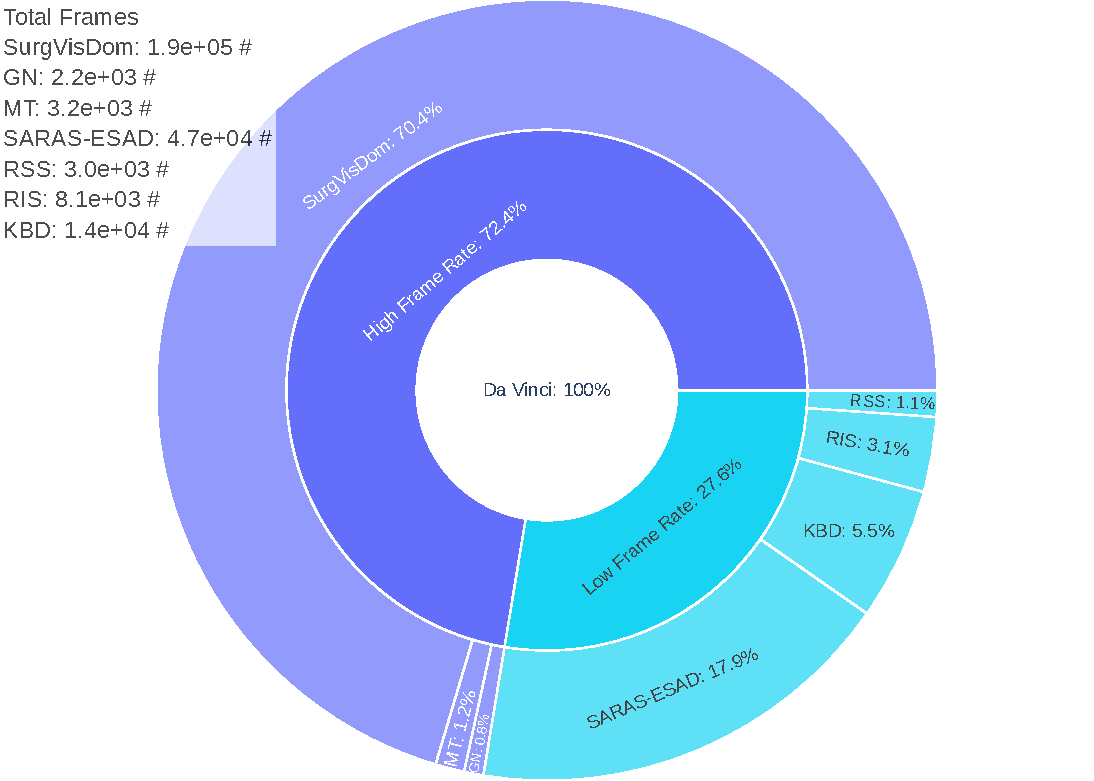
\includegraphics[width=0.8\textwidth]{fig/fig_da_vinci.pdf}
    \caption{Da Vinci surgery datasets. Included are: \href{https://surgvisdom.grand-challenge.org/}{SurgVisDom} \cite{zia2021surgical}, \href{http://hamlyn.doc.ic.ac.uk/vision/}{GN} \cite{giannarou2012probabilistic}, \href{http://hamlyn.doc.ic.ac.uk/vision/}{MT} \cite{mountney2010three}, \href{https://saras-esad.grand-challenge.org/}{SARAS-ESAD} \cite{bawa2020esad}, \href{https://endovissub2017-kidneyboundarydetection.grand-challenge.org/}{KBD} \cite{hattab2020kidney}, \href{https://endovissub2017-roboticinstrumentsegmentation.grand-challenge.org/}{RIS} \cite{allan20192017}, \href{https://endovissub2018-roboticscenesegmentation.grand-challenge.org/home/}{RSS} \cite{allan20202018}}
    \label{c3:fig:data_a}
\end{subfigure}
\begin{subfigure}[b]{\textwidth}
    \centering
    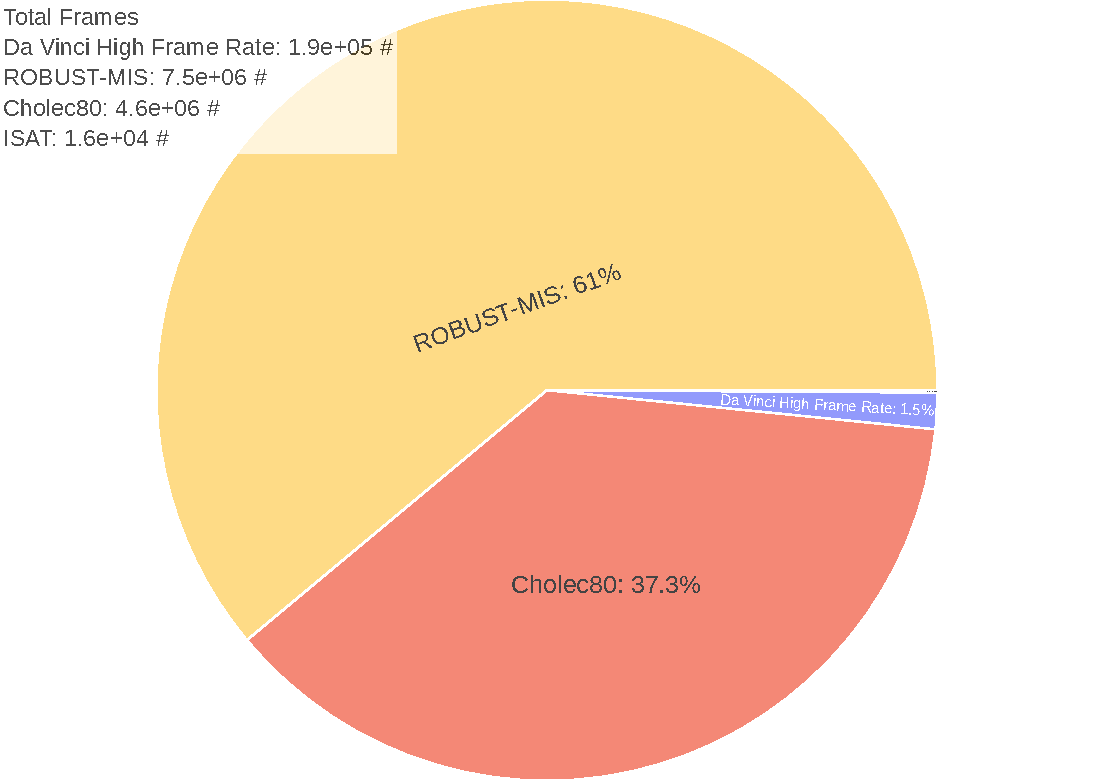
\includegraphics[width=0.8\textwidth]{fig/fig_da_vinci_high_fps_laparoscopic.pdf}
    \caption{Laparoscopic datasets and HFR da Vinci dataset from (a) for comparison. Included are: \href{https://robustmis2019.grand-challenge.org/}{ROBUST-MIS} \cite{maier2020heidelberg}, \href{http://camma.u-strasbg.fr/datasets}{Cholec80} \cite{twinanda2016endonet}, \href{https://endovissub-instrument.grand-challenge.org/}{ISAT} \cite{bodenstedt2018comparative}.}
    \label{c3:fig:data_b}
\end{subfigure}    
\caption{Da Vinci surgery and laparoscopic surgery datasets. Shown are relative sizes and the absolute number of frames. Da Vinci surgery datasets are often released at a low frame rate of $1\,\text{fps}$ for segmentation tasks (a). Much more laparoscopic surgery data is available (b).}
\label{c3:fig:data}
\end{figure}

\subsubsection{Da Vinci Surgery Data Pre-Processing}

Many of the da Vinci surgery datasets are designed for tool or tissue segmentation tasks, therefore, they are published at a frame rate of $1\,\text{fps}$, see \figref{c3:fig:data_a}. We merge all high frame rate (HFR) datasets into a single dataset and manually remove image sequences with camera motion, which amount to $5\%$ of all
HFR data. We crop the remaining data to remove status indicators, and scale the images to $306\times408$ pixels, later to be cropped by the \textit{homography generation algorithm} to a resolution of $240\times320$.

\subsubsection{Laparoscopic Surgery Data Pre-Processing}
\label{c3:sec:lap_pre}

Laparoscopic images are typically observed through a Hopkins telescope, which causes a black circular boundary in the view, see \figref{c3:fig:seg}. This boundary does not exist in da Vinci surgery recordings. For inference on the laparoscopic surgery image sequences, the most straightforward approach is to crop the view. To this purpose, we determine the center and radius of the circular boundary, which is only partially visible. We detect it by randomly sampling $N$ points $\mathbf{p}_i = (u_i,v_i)^\text{T}$ on the boundary. This is similar to work in \cite{munzer2013detection}, but instead of computing an analytical solution, we fit a circle by means of a least squares solution through inversion of
\begin{equation}
    \begin{bmatrix}
        2u_0     & 2v_0     & 1 \\
                 & \vdots   & \\
        2u_{N-1} & 2v_{N-1} & 1
    \end{bmatrix}
    \begin{bmatrix}
        x_0 \\ x_1 \\ x_2
    \end{bmatrix} = 
    \begin{bmatrix}
        u_0^2 + v_0^2 \\
        \vdots        \\
        u_{N-1}^2 + v_{N-1}^2
    \end{bmatrix},
\end{equation}
where the circle's center is $(x_0, x_1)$, and its radius is $\sqrt{x_2 + x^2_0 + x^2_1}$. We then crop the view centrally around the circle's center, and scale it to a resolution of $240\times320$. An implementation is provided on GitHub\footnote[2]{\url{https://github.com/RViMLab/endoscopy}}.

\begin{figure}[tb]
\centering
\begin{subfigure}[b]{\textwidth}
    \centering
    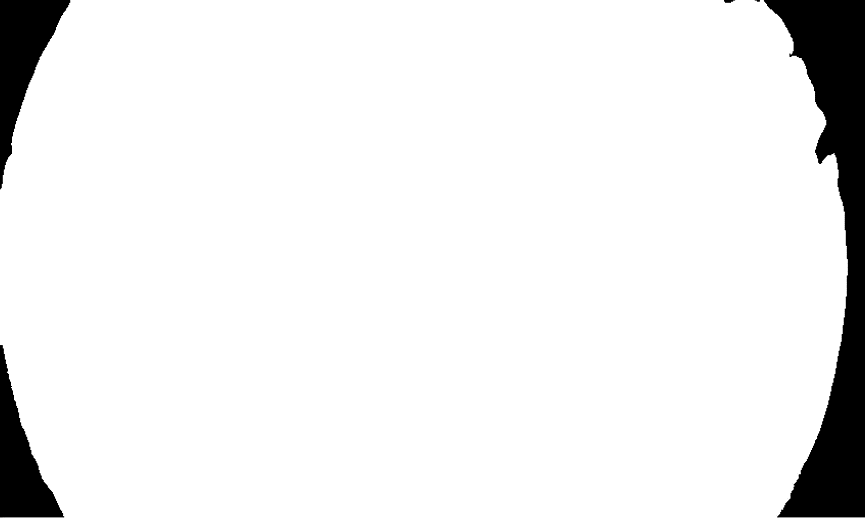
\includegraphics[width=0.8\textwidth]{img/annotation/annotation_seg.png}
    \caption{Binary segmentation mask, obtained through thresholding the bilateral filtered image.}
    \label{c3:fig:seg_a}
\end{subfigure}
\begin{subfigure}[b]{\textwidth}
    \centering
    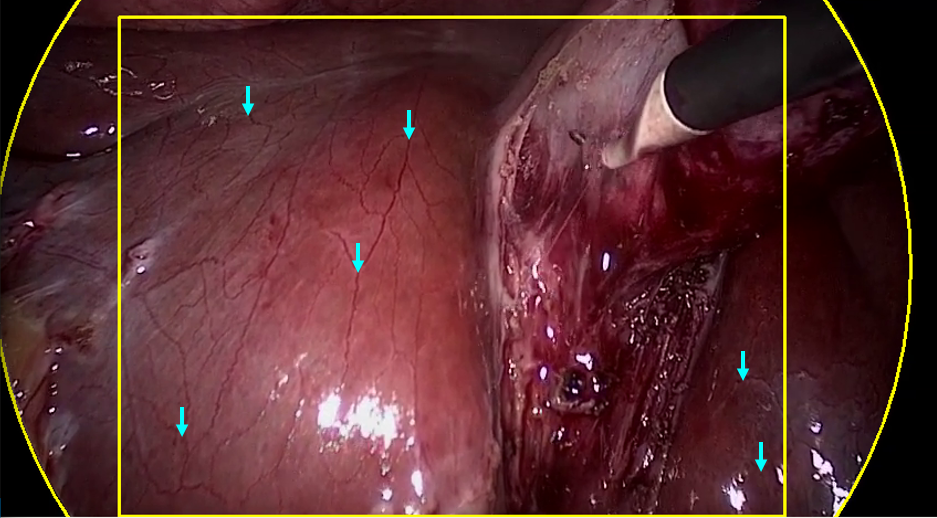
\includegraphics[width=0.8\textwidth]{img/annotation/annotation_real.png}
    \caption{Circular boundary detection and static landmarks (blue arrows).}
    \label{c3:fig:seg_b}
\end{subfigure}
\caption{Cholec80 dataset pre-processing, referring to \secref{c3:sec:lap_pre}. The black boundary circle is automatically detected. Landmarks are manually annotated and tracked over time (b).}
\label{c3:fig:seg}
\end{figure}

\subsubsection{Ground Truth Generation}
\label{c3:sec:gt_gen}
One can simply use the synthetically generated camera motion as ground truth at train time. For inference on the laparoscopic dataset, this is not possible. We therefore generate ground truth data by randomly sampling $50$ image sequences with $10$ frames each from the Cholec80 dataset. In these image sequences, we find characteristic landmarks that are neither subject to tool, nor to object motion, see \figref{c3:fig:seg_b}. Tracking of these landmarks over time allows one to estimate the camera motion in between consecutive frames through \eqref{c3:eq:hom_lin_sys}.

\subsection{Deep Homography Estimation}

In this work we exploit the static camera in da Vinci surgeries, which allows us to isolate camera motion free image sequences. The processing pipeline is shown in \figref{c3:fig:hom}.

Image pairs are sampled from image sequences of the HFR da Vinci surgery dataset of \figref{c3:fig:data_a}. An image pair consists of an anchor image $\mathcal{I}_n$, and an offset image $\mathcal{I}_{n+t}$. The offset image is sampled uniformly from and interval $t\in[-T,T]$ around the anchor. The HFR da Vinci surgery dataset is relatively small, compared to the laparoscopic datasets, see \figref{c3:fig:data_b}. Therefore, we apply image augmentations to the sampled image pairs. They include transform to grayscale, horizontal, and vertical flipping, cropping, change in brightness, and contrast, Gaussian blur, fog simulation, and random combinations of those. Camera motion is then added synthetically to the augmented image $\mathcal{I}^\text{aug}_{n+t}$ via the \textit{homography generation algorithm} from \secref{c3:sec:hom_gen}. A DNN, with a backbone, then learns to predict the homography $\mathbf{G}_{4\text{point}}$ between the augmented image, and the augmented image with synthetic camera motion at time step $n+t$.

%\begin{landscape}
\begin{figure}[tb]
    \centering
    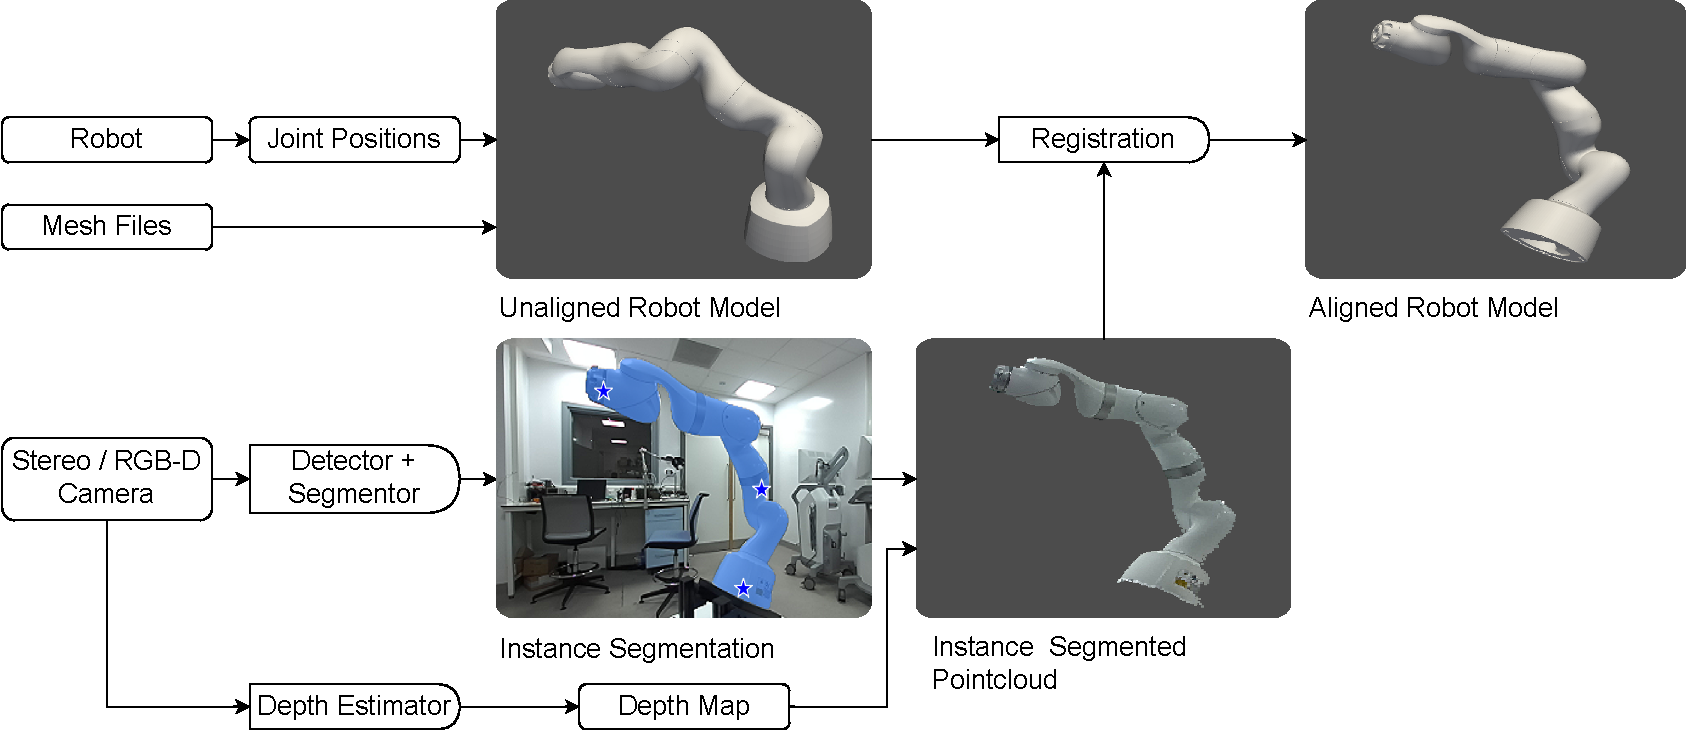
\includegraphics[width=\linewidth]{img/pipeline.pdf}
    \caption{Deep homography estimation training pipeline. Image pairs are sampled from the HFR da Vinci surgery dataset. The \textit{homography generation algorithm} then adds synthetic camera motion to the augmented images, which is regressed through a backbone DNN.}
    \label{c3:fig:hom}
\end{figure}
%\end{landscape}

\subsection{Homography Generation Algorithm}
\label{c3:sec:hom_gen}

In its core, the \textit{homography generation algorithm} is based on the works of \cite{detone2016deep}. However, where \citeauthor{detone2016deep} crop the image with a safety margin, our method allows to sample image crops across the entire image. Additionally, our method computes feasible homographies at runtime. This allows us to continuously generate synthetic camera motion, rather then training on a fixed set of precomputed homographies. The \textit{homography generation algorithm} is summarized in Alg.\,\ref{alg::hom}, and visualized in \figref{c3:fig:hom}.

Initially, a \textit{crop polygon} $\mathbb{P}_c$ is generated for the augmented image $\mathcal{I}^\text{aug}_n$. The \textit{crop polygon} is defined through a set of points in the augmented image $\mathbb{P}_c = \{\mathbf{p}^c_i,\,i\in \left[0,3\right]\}$, which span a rectangle. The top left corner $\mathbf{p}^c_0$ is randomly sampled such that the \textit{crop polygon} $\mathbb{P}_c$ resides within the image border polygon $\mathbb{P}_b$, hence $\mathbf{p}^c_0 \in ([0, h_b - h_c], [0, w_b - w_c])$, where $h$, and $w$ are the height and width of the \textit{crop}, and the \textit{border polygon}, respectively. Following that, a random four point homography $\mathbf{G}_{4\text{point}}$ \eqref{c3:eq:4pt} is generated by sampling edge deviations $\Delta u_i \land \Delta v_i \in [-\varrho, \varrho]$. The corresponding inverse homography $\mathbf{G}^{-1}$ is used to warp each point of the border polygon $\mathbb{P}_b$ to $\mathbb{P}^\prime_b$. Finally, the Dimensionally Extended 9-Intersection Model \cite{clementini1994modelling} is used to determine whether the warped polygon $\mathbb{P}^\prime_b$ contains $\mathbb{P}_c$, for which we utilize the Python library \textit{Shapely}\footnote[3]{\url{https://pypi.org/project/Shapely}}. If the thus found intersection matrix $\IM$ satisfies
\begin{equation}
    \IM(\mathbb{P}^\prime_b, \mathbb{P}_c) = \begin{bmatrix}
        T & * & * \\
        * & * & * \\
        F & F & *
    \end{bmatrix},
\end{equation}
the homography $\mathbf{G}^{-1}$ is returned, otherwise a new four point homograpy $\mathbf{G}_{4\text{point}}$ is sampled. Therein, $*$ indicates that the intersection matrix may hold any value, and $T,\,F$ indicate that the intersection matrix must be true or false at the respective position. In the unlikely case that no homography is found after \textit{maximum rollouts}, the identity $\mathbf{G}_{4\text{point}} = \mathbf{0}$ is returned. Once a suitable homography is found, a crop of the augmented image $\Crop(\mathcal{I}^\text{aug}_n, \mathbb{P}_c)$ is computed, as well as a crop of the warped augmented image at time $n+t$, $\Crop(\Warp(\mathcal{I}^\text{aug}_{n+t}, \mathbf{G}^{-1}), \mathbb{P}_c)$. This keeps all computationally expensive operations outside the loop.

\begin{algorithm}
    \SetAlgoLined
    Randomly sample crop polygon $\mathbb{P}_c$ of desired shape in $\mathbb{P}_b$\;
    \While{rollouts $<$ maximum rollouts}{
        Randomly sample $\mathbf{G}_{4\text{point}}$, where $\Delta u_i \land \Delta v_i \in \left[-\varrho, \varrho\right] \forall i$\;
        Perspective transform boundary polygon $p: \mathbb{P}_b, \mathbf{G}^{-1}\rightarrow\mathbb{P}^\prime_b$\;
        Compute intersection matrix $\IM(\mathbb{P}^\prime_b, \mathbb{P}_c)$\;
        \If{$\IM = \begin{bmatrix}T & * & * \\ * & * & * \\ F & F & *\end{bmatrix}$}{
            \Return{$\mathbf{G}_{4\text{point}}$, $\mathbb{P}_c$}\;
        }
        Increment \textit{rollouts}\;
    }
    \Return{$\mathbf{0}$, $\mathbb{P}_c$}\;
    \caption{Homography generation algorithm.}
    \label{alg::hom}
\end{algorithm}

\section{Experiments}
We train DNNs on a $80\%$ train split of the HFR da Vinci surgery dataset from \figref{c3:fig:data_a}. The $20\%$ test split is referred to as test set in the following. Inference is performed on the ground truth set from \secref{c3:sec:gt_gen}. We compute the Mean Pairwise Distance (MPD) of the predicted value for $\mathbf{G}_{4\text{point}}$ from the desired one. We then compute the Cumulative Distribution Function (CDF) of all MPDs. We evaluate the CDF at different thresholds $t_i,\,i\in\{30,50,70.90\}$, e.g. $30\%$ of all homography estimations are below a MPD of $t_{30}$. We additionally evaluate the compute time on a GeForce RTX 2070 GPU, and a Intel Core i7-9750H CPU.

\subsection{Backbone Search}
In this experiment, we aim to find the best performing backbone for homography estimation. Therefore, we run the same experiment repeatedly with fixed hyperparameters, and varying backbones. We train each network for $50$ epochs, with a batch size of $64$, using the Adam optimizer with a learning rate of $\num{2e-4}$. The edge devation $\varrho$ is set to $32$, and the sequence length $T$ to $25$.

\subsection{Homography Generation Algorithm}
In this experiment, we evaluate the \textit{homography generation algorithm}. For this experiment we fix the backbone to a ResNet-34, and train it for $100$ epochs, with a batch size of $256$, using the Adam optimizer with a learning rate of \num{1e-3}. Initially, we fix the sequence length $T$ to $25$, and train on different edge deviations $\varrho\in\{32,48,64\}$. Next, we fix the edge deviation $\varrho$ to $48$, and train on different sequence lengths $T\in\{1,25,50\}$, where a sequence length of $1$ corresponds to a static pair of images.

% Given the ResNet-34, which performs well on inference, and executes fast on the GPU, we run additional experiments to determine the effect of our method on homography estimation in dynamic surgical scenes. In this section, we train the ResNet-34 backbone for $100$ epochs, with a batch size of $256$, using the Adam optimizer with a learning rate of \num{1e-3}. Initially, we fix the sequence length $T$ to $25$, and train on different edge deviations $\varrho\in\{32,48,64\}$. Next, we fix the edge deviation $\varrho$ to $48$, and train on different sequence lengths $T\in\{1,25,50\}$, where a sequence length of $1$ corresponds to a static pair of images. The results are shown in \figref{c3:fig:resnet34}, and a qualitative example is presented in \figref{c3:fig:qualitative}.



\section{Results}

%In the following, the HFR da Vinci test set, and the Cholec80 annotated subset are referred to as test set, and inference set, respectively.   


%For the experiments, we use the HFR da Vinci surgery dataset, shown in \figref{c3:fig:data_a}, for training, and 


%We adjust the image resolution to $[240,\,320]$ for both datasets. We split the HFR da Vinci dataset into $20\%$ test, and $80\%$ training.

\subsection{Backbone Search}
\label{c3:sec:backbone_search}

% Previous work mainly relies on VGG-style DNN architectures. Our initial findings suggest that VGG-style DNNs perform badly at homography estimation. In the context of finding a better network, we evaluate different SOTA backbones across multiple compute regimes, see Tab.\,\ref{c3:tab::results}. 


% Each network is trained for $50$ epochs, with a batch size of $64$, using the Adam optimizer with a learning rate of $\num{2e-4}$. The edge devation $\varrho$ is set to $32$, and the sequence length $T$ to $25$.

The results are listed in Tab.\,\ref{c3:tab::results}. It can be seen that the deep methods generally outperform the classical methods on the test set. There is a tendency that models with more parameters perform better. On the ground truth set, this tendency vanishes. The differences in performance become independent of the number of parameters. Noticeably, many backbones still outperform the classical methods across all thresholds on the ground truth set, and low compute regime models also run quicker on CPU than comparable classical methods. E.g. we find that EfficientNet-B0, and RegNetY-400MF run at $36\,\text{Hz}$, and $50\,\text{Hz}$ on a CPU, respectively. Both outperform SURF \& RANSAC in homography estimation, which runs at $20\,\text{Hz}$.

%These findings make the backbone selection a matter of optimization for computational requirements. ResNet-34 is among the models with the best inference performance, and runs $6\,\text{ms}$ on GPU. For further investigation, we therefore select a ResNet-34 backbone. 

\begin{table}
\centering
\caption{Results referring to \secref{c3:sec:backbone_search}. All methods are tested on the da Vinci HFR test set, indicated by $t^\text{test}_i$, and the Cholec80 inference set, indicated by $t^\text{gt}_i$. Best, and second best metrics are highlighted with bold character. Improvements in precision $t^\text{gt}_{90,\text{imp}}$ and compute time $\text{CPU}_\text{imp}$ are given w.r.t. SURF \& RANSAC. \label{c3:tab::results}}
\begin{adjustbox}{angle=90, max height=0.9\textheight}
    \begin{tabular}{lrrrrrrrrrr} \toprule
        Name            & $t^\text{test}_{30}/t^\text{gt}_{30}\,[\text{pixels}]$ & $t^\text{test}_{50}/t^\text{gt}_{50}\,[\text{pixels}]$ & $t^\text{test}_{70}/t^\text{gt}_{70}\,[\text{pixels}]$ & $t^\text{test}_{90}/t^\text{gt}_{90}\,[\text{pixels}]$ & $t^\text{gt}_{90,\text{imp}}\,[\%]$ & $\text{params}\,[\text{M}]$ & $\text{flops}\,[\text{M}]$ & $\text{GPU}\,[\text{ms}]$ & $\text{CPU}\,[\text{ms}]$ & $\text{CPU}_\text{imp}\,[\%]$ \\ \midrule
        VGG-style       & $4.83/2.45         $ & $ 6.47/2.94         $ & $ 8.68/3.59         $ & $ 13.23/5.41                  $ & $- 60         $ & $92.92$ & $11.12$ & $ \mathbf{2} \pm 1$ & $83          \pm 2$ & $- 69          \pm 33$ \\
        ResNet-18       & $1.42/1.12         $ & $ 1.95/1.33         $ & $ 2.82/1.58         $ & $  5.06/2.20                  $ & $  35         $ & $11.19$ & $ 6.02$ & $ \mathbf{3} \pm 1$ & $31          \pm 3$ & $  38          \pm 13$ \\
        ResNet-34       & $1.33/\mathbf{1.02}$ & $ 1.81/\mathbf{1.19}$ & $ 2.56/\mathbf{1.52}$ & $  4.63/2.08                  $ & $  \mathbf{39}$ & $21.3 $ & $11.74$ & $ 6          \pm 1$ & $51          \pm 5$ & $-  3          \pm 23$ \\
        ResNet-50       & $1.40/1.08         $ & $ 1.89/1.33         $ & $ 2.70/1.57         $ & $  4.79/2.21                  $ & $  35         $ & $23.53$ & $13.12$ & $10          \pm 1$ & $72          \pm 4$ & $- 46          \pm 29$ \\
        EfficientNet-B0 & $1.36/1.09         $ & $ 1.83/1.31         $ & $ 2.62/\mathbf{1.50}$ & $  4.64/\mathbf{2.01}         $ & $  \mathbf{41}$ & $ 4.02$ & $ 1.28$ & $12          \pm 2$ & $28          \pm 2$ & $  43          \pm 12$ \\
        EfficientNet-B1 & $1.32/\mathbf{1.02}$ & $ 1.77/\mathbf{1.26}$ & $ 2.50/1.57         $ & $  4.42/\mathbf{2.01}         $ & $  \mathbf{41}$ & $ 6.52$ & $ 1.88$ & $17          \pm 1$ & $37          \pm 1$ & $  25          \pm 15$ \\
        EfficientNet-B2 & $1.40/1.06         $ & $ 1.85/1.29         $ & $ 2.57/1.55         $ & $  4.42/2.15                  $ & $  37         $ & $ 7.71$ & $ 2.16$ & $17          \pm 2$ & $41          \pm 1$ & $  18          \pm 16$ \\
        EfficientNet-B3 & $1.31/1.05         $ & $ 1.75/1.36         $ & $ 2.44/1.68         $ & $  4.23/2.26                  $ & $  33         $ & $10.71$ & $ 3.14$ & $20          \pm 2$ & $55          \pm 4$ & $- 11          \pm 23$ \\
        EfficientNet-B4 & $\mathbf{1.23}/1.08$ & $ \mathbf{1.65}/1.31$ & $ \mathbf{2.29}/1.69$ & $  \mathbf{4.02}/2.14         $ & $  37         $ & $17.56$ & $ 4.88$ & $24          \pm 2$ & $68          \pm 5$ & $- 38          \pm 29$ \\
        EfficientNet-B5 & $1.26/1.18         $ & $ 1.67/1.35         $ & $ \mathbf{2.30}/1.65$ & $  \mathbf{4.02}/\mathbf{2.06}$ & $  \mathbf{39}$ & $28.36$ & $ 7.62$ & $29          \pm 2$ & $93          \pm 5$ & $- 89          \pm 37$ \\
        RegNetY-400MF   & $1.55/\mathbf{1.01}$ & $ 2.07/1.29         $ & $ 2.90/1.60         $ & $  5.08/2.12                  $ & $  37         $ & $ 3.91$ & $ 1.32$ & $13          \pm 1$ & $\mathbf{20} \pm 1$ & $  \mathbf{58} \pm  8$ \\
        RegNetY-600MF   & $1.47/1.03         $ & $ 1.98/1.28         $ & $ 2.80/1.56         $ & $  4.87/2.21                  $ & $  35         $ & $ 5.45$ & $ 1.94$ & $13          \pm 1$ & $24          \pm 3$ & $  52          \pm 11$ \\
        RegNetY-800MF   & $1.43/1.08         $ & $ 1.92/1.32         $ & $ 2.70/1.59         $ & $  4.76/2.12                  $ & $  37         $ & $ 5.50$ & $ 2.54$ & $12          \pm 1$ & $24          \pm 1$ & $  51          \pm 10$ \\
        RegNetY-1.6GF   & $1.38/1.03         $ & $ 1.83/1.27         $ & $ 2.52/1.60         $ & $  4.35/2.16                  $ & $  36         $ & $10.32$ & $ 5.08$ & $21          \pm 2$ & $42          \pm 4$ & $  16          \pm 18$ \\
        RegNetY-4.0GF   & $1.27/1.05         $ & $ 1.69/\mathbf{1.26}$ & $ 2.36/1.66         $ & $  4.17/2.17                  $ & $  36         $ & $19.57$ & $12.36$ & $21          \pm 2$ & $66          \pm 5$ & $- 34          \pm 28$ \\
        RegNetY-6.4GF   & $\mathbf{1.21}/1.04$ & $ \mathbf{1.64}/1.27$ & $ 2.32/1.60         $ & $  4.17/2.09                  $ & $  38         $ & $29.30$ & $19.72$ & $25          \pm 3$ & $98          \pm 6$ & $-100          \pm 40$ \\
        SURF \& RANSAC  & $4.06/1.07         $ & $ 5.65/1.40         $ & $ 7.93/2.02         $ & $ 13.62/3.39                  $ & $   0         $ & N/A     & N/A     &  N/A                & $49          \pm 9$ & $   0          \pm 27$ \\
        SIFT \& RANSAC  & $4.28/1.25         $ & $ 6.02/1.76         $ & $ 8.65/2.48         $ & $ 16.52/4.63                  $ & $- 37         $ & N/A     & N/A     &  N/A                & $37          \pm 9$ & $  25          \pm 22$ \\
        ORB \& RANSAC   & $6.52/1.65         $ & $10.48/2.47         $ & $20.12/3.71         $ & $122.66/6.81                  $ & $-101         $ & N/A     & N/A     &  N/A                & $\mathbf{12} \pm 2$ & $  \mathbf{76} \pm  6$ \\ \bottomrule
    \end{tabular}
\end{adjustbox}
\end{table}
\subsection{Homography Generation Algorithm}
\label{c3:sec:hom_opt}

% Given the ResNet-34, which performs well on inference, and executes fast on the GPU, we run additional experiments to determine the effect of our method on homography estimation in dynamic surgical scenes. In this section, we train the ResNet-34 backbone for $100$ epochs, with a batch size of $256$, using the Adam optimizer with a learning rate of \num{1e-3}. Initially, we fix the sequence length $T$ to $25$, and train on different edge deviations $\varrho\in\{32,48,64\}$. Next, we fix the edge deviation $\varrho$ to $48$, and train on different sequence lengths $T\in\{1,25,50\}$, where a sequence length of $1$ corresponds to a static pair of images. The results are shown in \figref{c3:fig:resnet34}, and a qualitative example is presented in \figref{c3:fig:qualitative}.

\begin{figure}[tb]
\centering
\begin{subfigure}[b]{\textwidth}
    \centering
    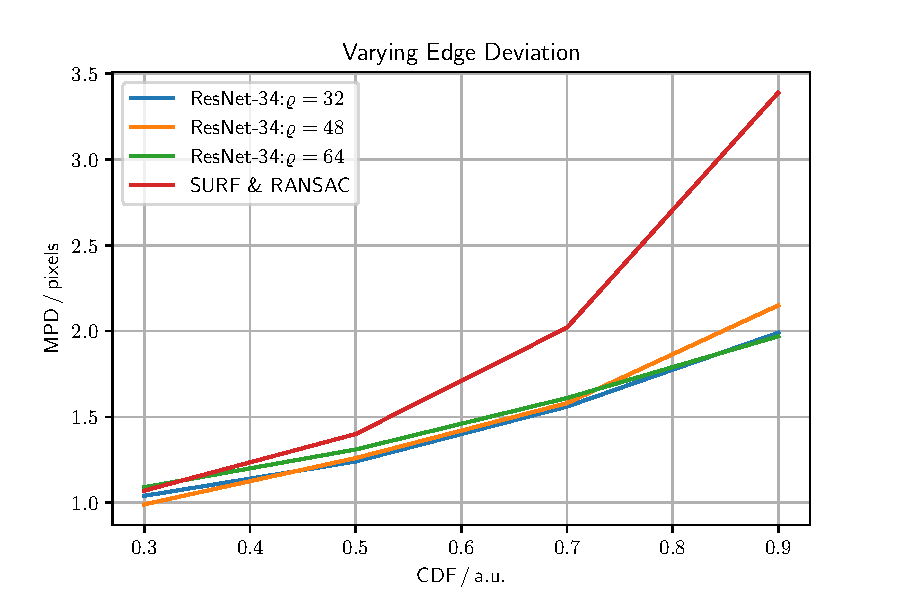
\includegraphics[width=0.8\textwidth]{fig/frac/var_rho.pdf}
    \caption{Varying edge deviation $\varrho\in\{32,48,64\}$, and fixed sequence length $T=25$.}
    \label{c3:fig:resnet34_a}
\end{subfigure}
\begin{subfigure}[b]{\textwidth}
    \centering
    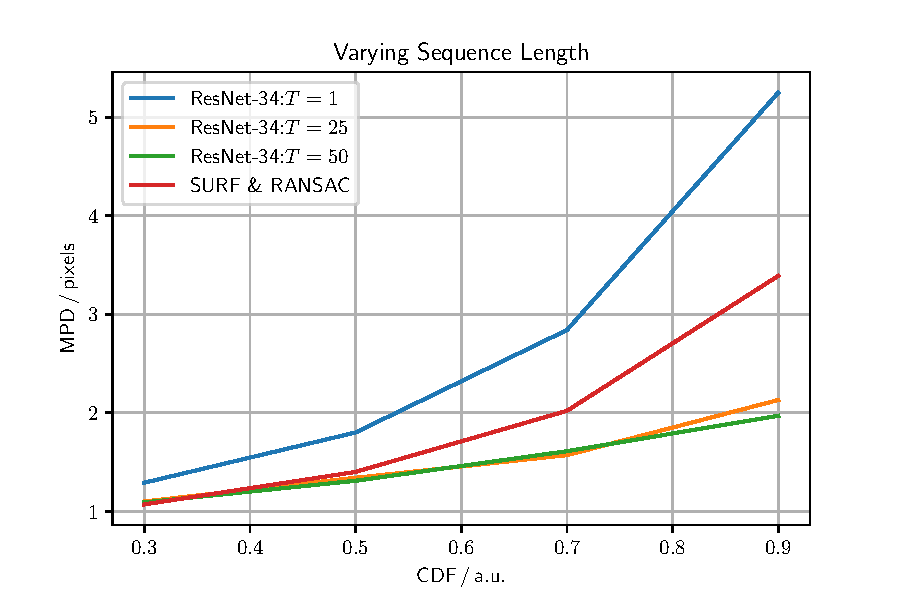
\includegraphics[width=0.8\textwidth]{fig/frac/var_seq.pdf}
    \caption{Varying sequence length $T\in\{1,25,50\}$, and fixed edge deviation $\varrho=48$.}
    \label{c3:fig:resnet34_b}
\end{subfigure}
\caption{Homography generation optimization, referring to \secref{c3:sec:hom_opt}. Shown is a ResNet-34 homography estimation for different homography generation configurations, and a SURF \& RANSAC homography estimation for reference. The edge deviation $\varrho$ is varied in (a), and the sequence length $T$ is varied in (b).}
\label{c3:fig:resnet34}
\end{figure}

\begin{figure}[tb]
\centering
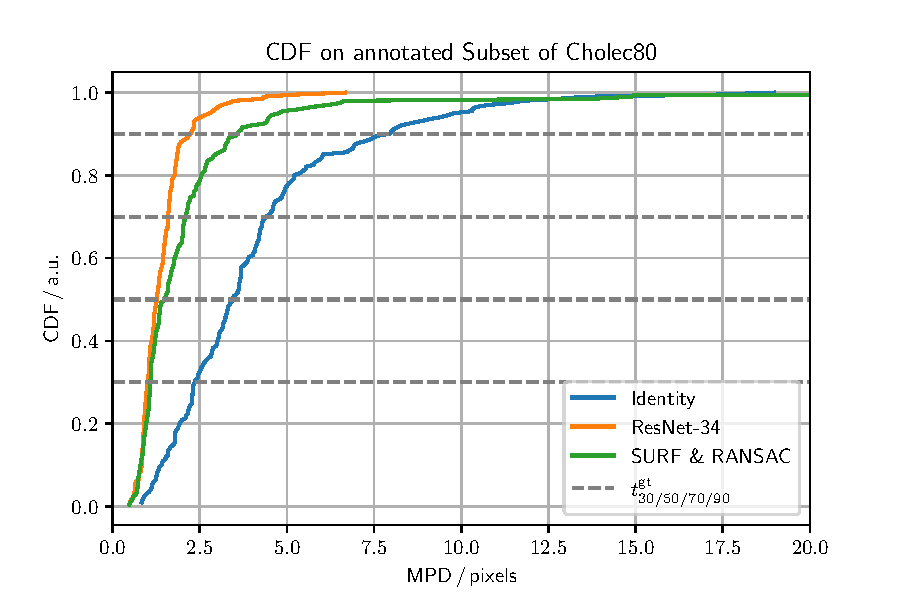
\includegraphics[width=\textwidth]{fig/frac/cdf.pdf}
\caption{CDF for SURF \& RANSAC, and ResNet-34, trained with a sequence length $T=25$, and edge deviation $\varrho=48$. The identity is added for reference. CDF thresholds for the SURF \& RANSAC are $t^\text{gt}_{1/10/30/50/70/90} = 0.51/0.80/1.09/1.48/2.07/3.53\,\text{pixels}$, and for the ResNet-34 $t^\text{gt}_{1/10/30/50/70/90} = 0.50/0.83/1.00/1.26/1.59/2.15\,\text{pixels}$. ResNet-34 generally performs better, and has no outliers.}
\label{c3:fig:resnet34_c}
\end{figure}

% Given the ResNet-34, which performs well on inference, and executes fast on the GPU, we run additional experiments to determine the effect of our method on homography estimation in dynamic surgical scenes. In this section, we train the ResNet-34 backbone for $100$ epochs, with a batch size of $256$, using the Adam optimizer with a learning rate of \num{1e-3}. Initially, we fix the sequence length $T$ to $25$, and train on different edge deviations $\varrho\in\{32,48,64\}$. Next, we fix the edge deviation $\varrho$ to $48$, and train on different sequence lengths $T\in\{1,25,50\}$, where a sequence length of $1$ corresponds to a static pair of images. The results are shown in \figref{c3:fig:resnet34}, and a qualitative example is presented in \figref{c3:fig:qualitative}.

Given that ResNet-34 performs well on the ground truth set, and executes fast on the GPU, we run the \textit{homography generation algorithm} experiments with it. It can be seen in \figref{c3:fig:resnet34_a}, that the edge deviation $\varrho$ is neglectable for inference. In \figref{c3:fig:resnet34_b}, one sees the effects of the sequence length $T$ on the inference performance. Notably, with $T=1$, corresponding to static image pairs, the SURF \& RANSAC homography estimation outperforms the ResNet-34. For the other sequence lengths, ResNet-34 outperforms the classical homography estimation. The CDF for the best performing combination of parameters, with $T=25$, and $\varrho=48$, is shown in \figref{c3:fig:resnet34_c}. Our method generally outperforms SURF \& RANSAC. The advantage of our method becomes most apparent for a $\text{CDF}\geq0.5$. Even the identity outperforms SURF \& RANSAC for large MPDs. This aligns with the qualitative observation that motion is often overestimated by SURF \& RANSAC, which is shown in \figref{c3:fig:qualitative}. An exemplary video is provided\footnote{\url{https://drive.google.com/file/d/1totjHbhIMEL7a-QAiL7B1rT44wvWB6lO/view?usp=sharing}}.

% It can be seen in \figref{c3:fig:resnet34_a}, that the effect of the edge deviation $\varrho$ is neglectable for inference. This is because the motion in the inference set does not exceed the motion in the training set. In \figref{c3:fig:resnet34_b}, one sees the effects of the sequence length $T$ on the inference performance. Notably, with $T=1$, corresponding to static image pairs, the SURF \& RANSAC homography estimation outperforms the ResNet-34. For the other sequence lengths, ResNet-34 outperforms the classical homography estimation, validating our method. The CDF for the best performing combination of parameters, with $T=25$, and $\varrho=48$, is shown in \figref{c3:fig:resnet34_c}. Our method generally outperforms SURF \& RANSAC. The advantage of our method becomes most apparent for $\text{CDF}\geq0.5$. Even the identity outperforms SURF \& RANSAC for large MPD. This aligns with the qualitative observation that motion is often overestimated by SURF \& RANSAC, which is shown in \figref{c3:fig:qualitative}. 


% $\text{ResNet-34}$      - 0.50/0.83/1.00/1.26/1.59/2.15
% $\text{SURF \& RANSAC}$ - 0.51/0.80/1.09/1.48/2.07/3.53

%\begin{figure}[tb]
%    \centering
%    \resizebox{0.8\linewidth}{!}{
%        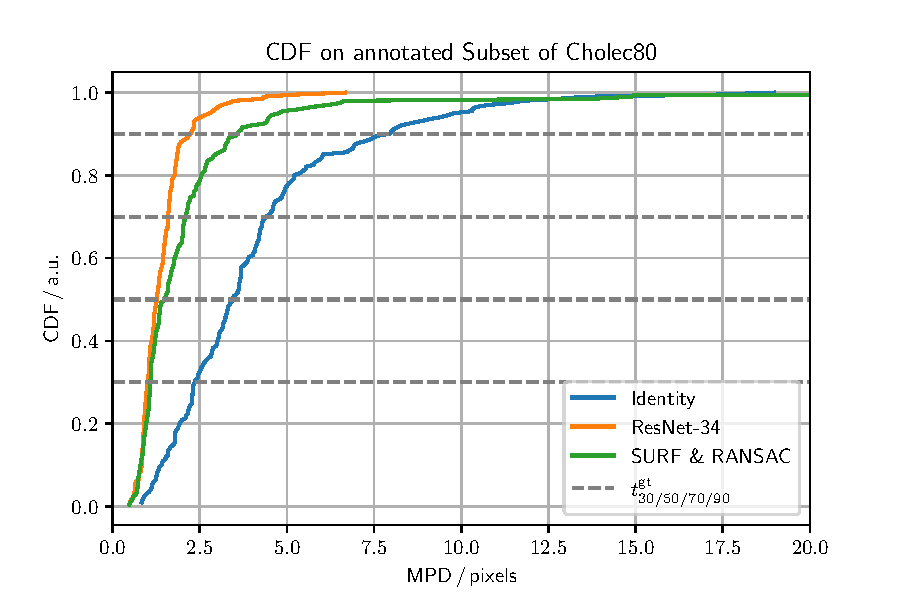
\includegraphics{fig/frac/cdf.pdf}
%    }
%    \caption{Caption}
%    \label{c3:fig:cdf}
%\end{figure}


% qualitative classical tends to overestimate motion
\begin{landscape}
\begin{figure}[tb]
\centering
\begin{subfigure}[b]{0.3\textwidth}
    \centering
    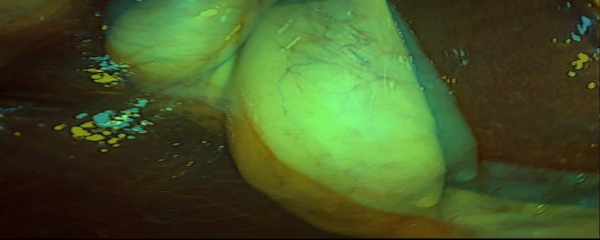
\includegraphics[width=0.3\textwidth]{img/homography_blends/blend_identity_strong_motion.png}
    \caption{Identity}
\end{subfigure}
\begin{subfigure}[b]{0.3\textwidth}
    \centering
    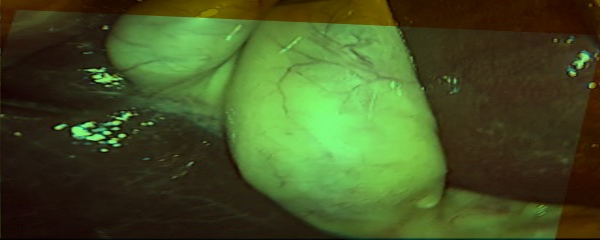
\includegraphics[width=0.3\textwidth]{img/homography_blends/blend_surf_strong_motion.png}
    \caption{SURF \& RANSAC}
\end{subfigure}
\begin{subfigure}[b]{0.3\textwidth}
    \centering
    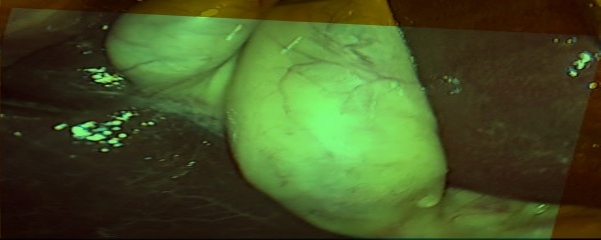
\includegraphics[width=0.3\textwidth]{img/homography_blends/blend_resnet_34_strong_motion.png}
    \caption{ResNet-34}
\end{subfigure}
\begin{subfigure}[b]{0.5\textwidth}
    \centering
    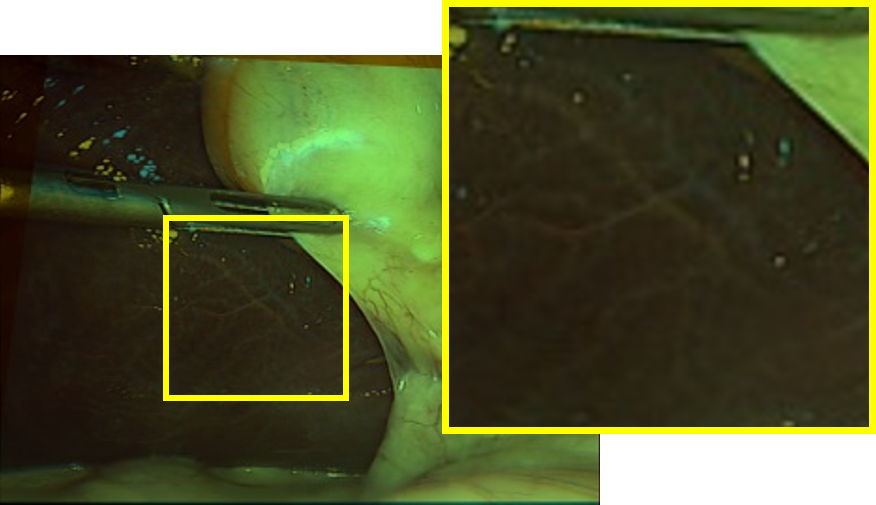
\includegraphics[width=0.5\textwidth]{img/homography_blends/blend_surf_zoom.png}
    \caption{Object Motion - SURF \& RANSAC, zoom}
\end{subfigure}
\begin{subfigure}[b]{0.5\textwidth}
    \centering
    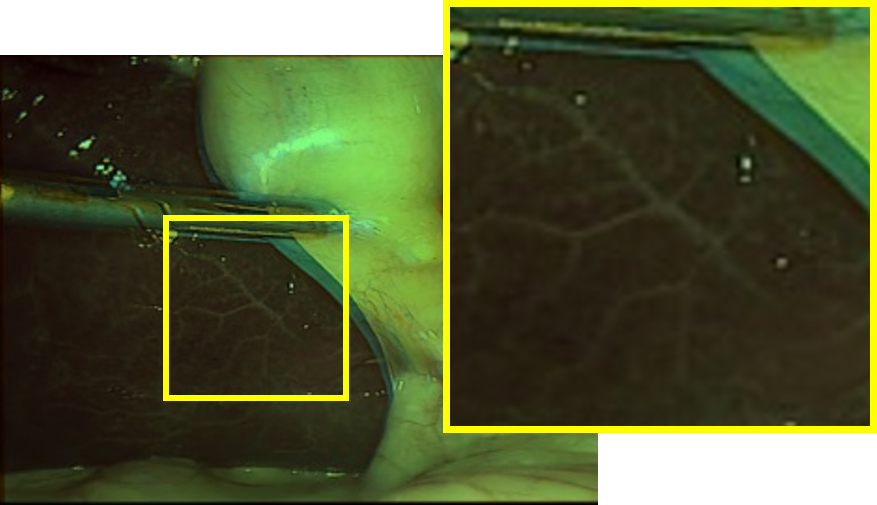
\includegraphics[width=0.5\textwidth]{img/homography_blends/blend_resnet_34_zoom.png}
    \caption{Object Motion - ResNet-34, zoom}
\end{subfigure}
\caption{Classical homography estimation using a SURF feature detector under RANSAC outlier rejection, and the proposed deep homography estimation with a ResNet-34 backbone, referring to \secref{c3:sec:hom_opt}. Shown are blends of consecutive images from a $5\,\text{fps}$ resampled Cholec80 exemplary sequence \cite{twinanda2016endonet}. Decreasing the framerate from originally $25\,\text{fps}$ to $5\,\text{fps}$, increases the motion in between consecutive frames. (Top row) Homography estimation under predominantly camera motion. Both methods perform well. (Bottom row) Homography estimation under predominantly object motion. Especially in the zoomed images it can be seen that the classical method (d) misaligns the stationary parts of the image, whereas the proposed method (e) aligns the background well.}
\label{c3:fig:qualitative}
\end{figure}
\end{landscape}

%\url{https://drive.google.com/file/d/1totjHbhIMEL7a-QAiL7B1rT44wvWB6lO/view?usp=sharing} %<- submission
%\url{https://drive.google.com/file/d/17fmhSsPq290PuLXmtO-aWwo3KN4QkZA8/view?usp=sharing}
%\url{https://drive.google.com/file/d/1SpUtSVgwo_PAwAjULF-Ky_5CxRuhMYlm/view?usp=sharing}


\section{Discussion}

% summarize work
In this work we supervisedly learn homography estimation in dynamic surgical scenes. We train our method on a newly acquired, synthetically modified da Vinci surgery dataset and successfully cross the domain gap to videos of laparoscopic surgeries. To do so, we introduce extensive data augmentation and continuously generate synthetic camera motion through a novel \textit{homography generation algorithm}.

% highlight results and draw conclusions
In \secref{c3:sec:backbone_search}, we find that, despite the domain gap for the ground truth set, DNNs outperform classical methods, which is indicated in Tab.\,\ref{c3:tab::results}. The homography estimation performance proofs to be independent of the number of model parameters, which indicates an overfit to the test data. The independence of the number of parameters allows to optimize the backbone for computational requirements. E.g., a typical laparoscopic setup runs at $25-30\,\text{Hz}$, the classical method would thus already introduce a bottleneck at $20\,\text{Hz}$. On the other hand, EfficientNet-B0, with $36\,\text{Hz}$, and RegNetY-400MF, with $50\,\text{Hz}$, introduce no latency, and could be integrated into systems without GPU.

% In \secref{c3:sec:backbone_search}, we evaluate SOTA DNNs on homography estimation in dynamic surgical scenes. Despite the domain gap, we find that DNNs outperform classical methods, which is indicated in Tab.\,\ref{c3:tab::results}. It can further be seen that the homography estimation performance is independent of the DNN's number of parameters. This allows to directly optimize the backbone for computational requirements. E.g. in the low compute regime, we find that EfficientNet-B0, and RegNetY-400MF run at $36\,\text{Hz}$, and $50\,\text{Hz}$ on a CPU, respectively. Both outperform SURF \& RANSAC in homography estimation, which runs at $20\,\text{Hz}$. Typical laparoscopic setups run at $25-30\,\text{Hz}$, the classical method would thus already introduce a bottleneck. EfficientNet-B0, and RegNetY-400MF, on the other hand, would not, and could be integrated into systems without GPU.

In \secref{c3:sec:hom_opt}, we find that increasing the edge deviation has no effect on the homography estimation, see \figref{c3:fig:resnet34_a}. This is because the motion in the ground truth set does not exceed the motion in the training set. In \figref{c3:fig:resnet34_b}, we further find how training DNNs on synthetically modified da Vinci surgery image sequences enables our method to isolate camera from object and tool motion, validating our method. In \figref{c3:fig:resnet34_c}, it is demonstrated that ResNet-34 generally outperforms SURF \& RANSAC. This shows that generating camera motion synthetically through homographies, which approximates the surgical scene as a plane, does not pose an issue.

% In \secref{c3:sec:hom_opt}, we evaluate hyperparameters for the synthetic camera motion generation. The assumption that the surgical scene transforms as a plane might only be locally correct. However, we find that this does not pose an issue, and that our method estimates homographies across the entire range of camera motions well, see Fig.\ref{c3:fig:qualitative}. In \figref{c3:fig:resnet34}, we further find how training DNNs on synthetically modified da Vinci surgery image sequences enables our method to isolate camera from object and tool motion.

The object, and tool motion invariant camera motion estimation allows one to extract a laparoscope holder's actions from videos of laparoscopic interventions, which enables the generation of image-action-pairs. In future work, we will generate image-action-pairs from laparoscopic datasets and apply IL to them. Describing camera motion (actions) by means of a homography is grounded in recent research for robotic control of laparoscopes \cite{huber2021homographybased}. This work will therefore support the transition towards robotic automation approaches. It might further improve augmented reality, and image mosaicing methods in dynamic surgical environments.

